\chapter{Eigenvectors and Eigenvalues}


Like many specialized disciplines, Linear Algebra uses many unfamiliar terms whose origin you might wonder about. Eigenvectors and eigenvalues are two of them. If you know German, you’ll recognize that eigen means inherent or a characteristic attribute. Named by the German mathematician David Hilbert, an eigenvector mathematically describes a characteristic feature of an object, that remains unchanged after transformation. You can think of an eigenvector as the direction that doesn’t change direction. 

Eigenvalues and eigenvectors are a way to break down matrices that can simplify many calculations and enable us to understand various properties of the matrix. They are widely used in physics and engineering for stability analysis, vibration analysis, and many other applications. \index{eigenvector} \index{eigenvalue}

Let’s look at a visual example.

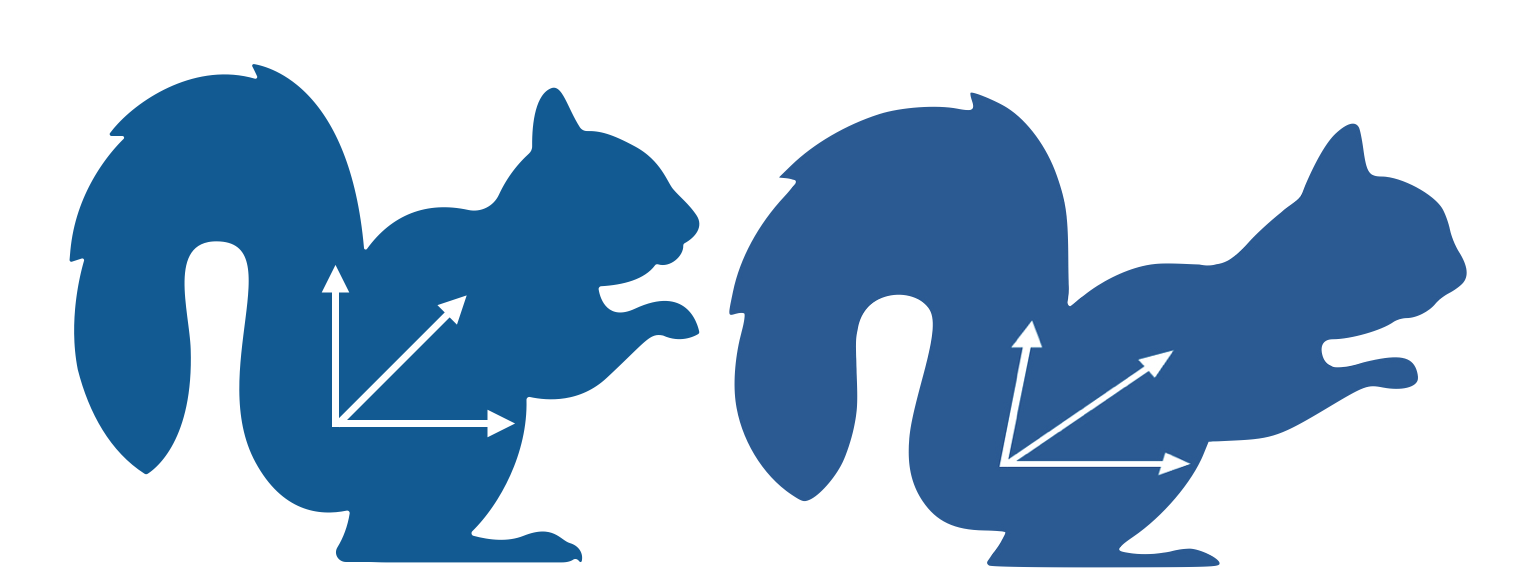
\includegraphics[width=0.8\textwidth]{EigenSquirrel.png}

You can see that the  image on the right is a skewed version of the image on the left. Look closely at the vectors and you’ll notice that the one of the vectors is pointing in the same direction in both images, while the direction of the other two vectors has changed. The eigenvector is the one at the bottom that points 0 degrees (or you can think of due east) in both images. Thus the characteristic attribute of both images is their horizontal direction.

When you overlay the vectors from one image over the other, you’ll notice that the horizontal vector, while the same direction in both images, is a bit longer in the skewed version. The scale of the stretch is described by an eigenvalue.

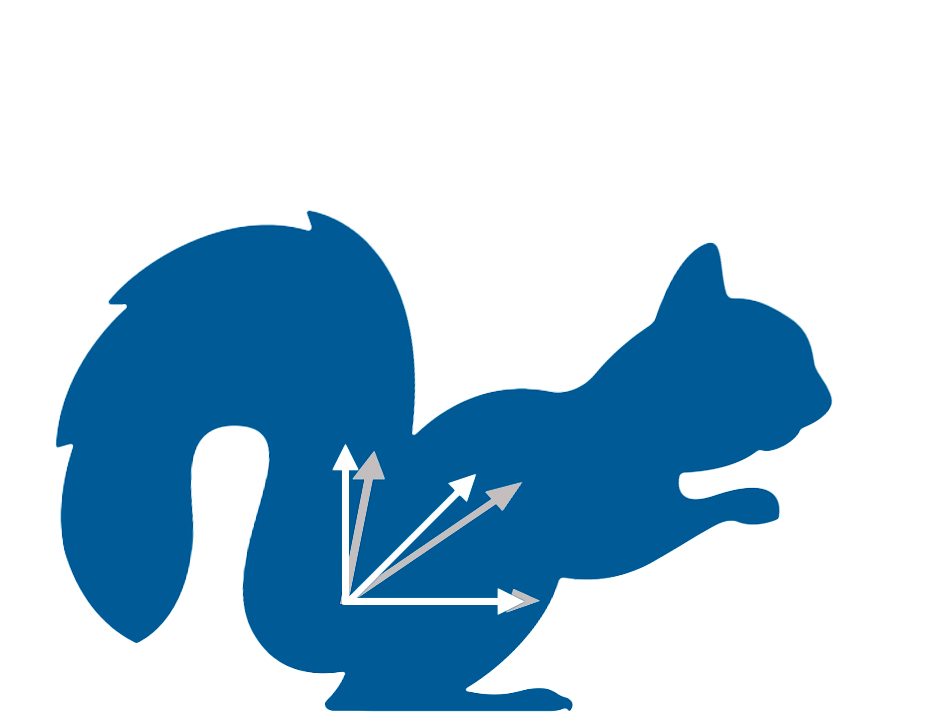
\includegraphics[width=0.4\textwidth]{OverlaySquirrel.png}


\section{Definition}

Given a square matrix $A$, a non-zero vector $v$ is an eigenvector of
$A$ if multiplying $A$ by $v$ results in a scalar multiple of $v$,
i.e.,

\begin{equation}
Av = \lambda v
\end{equation}

where $\lambda$ is a scalar known as the eigenvalue corresponding to the eigenvector $v$.

\section{Finding Eigenvalues and Eigenvectors}

You find the eigenvalues of a matrix $A$  by solving the characteristic equation:

\begin{equation}
\text{det}(A - \lambda I) = 0
\end{equation}

where $\text{det}(.)$ denotes the determinant, $I$ is the identity
matrix of the same size as $A$, and $\lambda$ is a scalar.

Once your find the eigenvalues, you can find the corresponding eigenvectors by substituting each eigenvalue into the equation $Av = \lambda
v$, and solving for $v$.

\section{Example}

For a $2 \times 2$ matrix $A = \begin{pmatrix} a & b \\ c &
  d \end{pmatrix}$, the characteristic equation is:

\begin{equation}
(a - \lambda)(d - \lambda) - bc = 0
\end{equation}

Solving this equation  gives the eigenvalues. Substituting each
eigenvalue back into the equation $Av = \lambda v$ gives the
corresponding eigenvectors.

Let matrix $A$ =
$$\begin{bmatrix}
5,4 &\\
 1,2& 
\end{bmatrix} $$

The characteristic equation is: 
$$|A - \lambda I| = 0$$ 
$$\begin{bmatrix}
5 - \lambda,4 &\\
 1,2- \lambda& 
\end{bmatrix} = 0$$
$$(5 - \lambda) (2 - \lambda) - (4)(1) = 0$$
$$10 - 5\lambda - 2\lambda + \lambda2 - 4 = 0$$
$$\lambda2 - 7\lambda + 6 = 0$$
$$(\lambda - 6)(\lambda - 1) = 0$$
$$\lambda = 6, \lambda = 1$$
Now that you have the eigen values you can substitue these values into the equation: 
$$|A - \lambda I| = 0$$ 
For $λ = 1$:
$$(A - \lambda I) v = O$$
$$\begin{bmatrix}
5-1, 4 &  \\
 1, 2-1& 
\end{bmatrix}
\begin{bmatrix}
x&  \\
 y& 
\end{bmatrix} = 
\begin{bmatrix}
0&  \\
0& 
\end{bmatrix}$$
$$\begin{bmatrix}
4, 4 &  \\
 1, 1& 
\end{bmatrix}
\begin{bmatrix}
x&  \\
 y& 
\end{bmatrix} = 
\begin{bmatrix}
0&  \\
0& 
\end{bmatrix}$$
Next,use elementary row transformation by multiplying row 2 by 4 and then subtracting row 1.
$$\begin{bmatrix}
4, 4 &  \\
 0, 0& 
\end{bmatrix}
\begin{bmatrix}
x&  \\
 y& 
\end{bmatrix} = 
\begin{bmatrix}
0&  \\
0& 
\end{bmatrix}$$
Now you can expand as an equation:
$$4x + 4y = 0$$
Assume y = w
$$4x = -4w$$
$$x = -w$$
The solution is:
$$\begin{bmatrix}
x&  \\
y& 
\end{bmatrix} = 
\begin{bmatrix}
-w&  \\
w& 
\end{bmatrix} = 
w\begin{bmatrix}
-1&  \\
1&
\end{bmatrix}$$
So the eigenvector is:
$$\begin{bmatrix}
-1&  \\
1&
\end{bmatrix}$$
Now we need to substitue the other eigenvalue, 6, into the equation and follow the same procedure for finding the eigenvector. 
$$\begin{bmatrix}
5-6, 4 &  \\
 1, 2-6& 
\end{bmatrix}
\begin{bmatrix}
x&  \\
 y& 
\end{bmatrix} = 
\begin{bmatrix}
0&  \\
0& 
\end{bmatrix}$$
$$\begin{bmatrix}
-1, 4 &  \\
 1, -4& 
\end{bmatrix}
\begin{bmatrix}
x&  \\
 y& 
\end{bmatrix} = 
\begin{bmatrix}
0&  \\
0& 
\end{bmatrix}$$
Next, use elementary row transformation by adding row 1 to row 2.
$$\begin{bmatrix}
-1, 4 &  \\
 0, 0& 
\end{bmatrix}
\begin{bmatrix}
x&  \\
 y& 
\end{bmatrix} = 
\begin{bmatrix}
0&  \\
0& 
\end{bmatrix}$$
Expand as an equation:
$$-x + 4y = 0$$
Assume y = w
$$-x + 4w = 0$$
$$x = 4w$$
The solution is:
$$\begin{bmatrix}
x&  \\
y& 
\end{bmatrix}=
\begin{bmatrix}
4w&  \\
w& 
\end{bmatrix} =
w\begin{bmatrix}
4&  \\
1& 
\end{bmatrix}$$
So the eigenvector is:
$$\begin{bmatrix}
4&  \\
1&
\end{bmatrix}$$
In conclusion, the eigenvectors of the given 2 x 2 matrix are:
$$\begin{bmatrix}
-1&  \\
1&
\end{bmatrix}
and \begin{bmatrix}
4&  \\
1&
\end{bmatrix}$$

\section{Eigenvalues and Eigenvectors in Python}
Create a file called \filename{vectors\_eigen.py} and enter this code:

\begin{Verbatim}
# import numpy to perform operations on vector
import numpy as np
from numpy.linalg import eig

a = np.array([[2, 2, 4], 
              [1, 3, 5],
              [2, 3, 4]])
eigenvalue,eigenvector = eig(a)

# The values are not in any particular order
print('Eigenvalues:', eigenvalue)

# The eig function returns the normalize vectors
print('Eigenvectors:', eigenvector)

\end{Verbatim}

\section{Where to Learn More}
Watch this video from Khan Academy,  Introduction to Eigenvectors: INSERT LINK